\documentclass{article}
\usepackage[margin=1in]{geometry}
\usepackage{amsmath}
\usepackage{setspace, fancyhdr, hyperref, xcolor, tikz, subcaption, float, marginnote, changebar}
\usepackage[normalem]{ulem}
\usetikzlibrary{fit}


\newcommand{\deleted}[1]{%
	\cbcolor{red}
	\begin{changebar}
		#1
	\end{changebar}%
}%

\newcommand{\added}[1]{%
	\cbcolor{green}
	\begin{changebar}
		#1
	\end{changebar}%
}%

\newcommand{\mycomment}[1]{
	{\color{red}\textsc{#1}}
}

\setlength{\changebarsep}{2ex}


\usetikzlibrary{positioning, intersections, calc, arrows}
\usepackage[square,numbers]{natbib}
\bibliographystyle{abbrvnat}
\newcommand{\comment}[1]{}
\newcommand{\thetitle}{Symbolic Manipulation and Computation in the Same Graph}

\pagestyle{fancy}
\fancyhf{}
\rhead{\thetitle}
\lhead{Darius Barbano}
\rfoot{Page \thepage}
\doublespacing

\author{Darius Barbano}
\title{\thetitle}
\date{}

\begin{document}
	
	\maketitle
	
	\newpage
	\tableofcontents
	\newpage
	
	\begin{abstract}
		
		\textcolor{red}{Rewritten abstract:}
		In theory, a neural network of sufficient size, where each neuron feeds the weighted sum of it's inputs through a sigmoid activation function, can approximate any function. In practice, these networks will become unnecesarily large to approximate many elementary functions, such as square root, absolute value, and logarithm functions. We propose a technique for introducing a wider range of functional classes in neural networks. \\
		
		General artificial intelligence refers to machine intelligence that performs a task as successfully as a human does. 
		
		\mycomment{The previous sentence does not make sense. How is \emph{general} AI defined in terms of the performance of \emph{one} task? }
		
		A fundamental difference between human neural network and current machine neural networks is that only human networks combine symbolic reasoning with computation. 
		
		\mycomment{This sentence needs support from the literature; otherwise, it is an opinion.}
		\\
		
		
		\sout{In order f}For neural networks to solve more complex problems, they must be able to manipulate representations of meaningful information. 
		
		\mycomment{The previous sentence is vague, in part because of ``weasel words''.\begin{enumerate}
				\item What do you mean by \emph{complex} in complex problems?
				\item What do you mean by \emph{meaningful} in meaningful information?
			\end{enumerate}
			Writing \emph{must} signifies that without the ability to represent symbols computers will not be able to solve more complex problems. I think that overstates the case.}\\
		
		While current networks have been largely successful in \sout{a variety of tasks from} image classification \sout{to}{\color{red}and} sentiment analysis, the internal computations of the networks have only consisted of many basic arithmetic operations. 
		
		\mycomment{\begin{enumerate}
				\item[] Why do you need the modifier \emph{current}?
				\item[] Be careful of the phrase from X to Y. It implies that X and Y are in the same metric space. Consider, for example, from NYC to Boston.
				\item[] I would not call a sigmoidal activation function a basic arithmetic operation. 
			\end{enumerate}
		}
		
		
		This model is effective in dealing with and taking advantage of relatively transparent patterns in the training data, but in no way does it attempt to develop meaningful representations of the data. 
		
		\mycomment{\begin{enumerate}
				\item[]  To which model does the modified \emph{this} refer? The one in this paper? One of the current neural networks you just mentioned?
				\item[] What does \emph{relatively transparent} mean?
				\item[] What, again, does \emph{meaningful} mean?
				\item[] What does \emph{effective} mean?
				\item[] The phrase \emph{taking advantage of} is anthropomorphic. You have not demonstrated that the neural networks you mentioned have intention. 
			\end{enumerate}
		}
		To build a model which generates new text based on some previously written text, modern networks would construct (through training) a framework which determines which word has the highest probability of logically making sense given the previous words in the text. These networks have no consideration for the meaning of the words chosen, only their probability of being correct as meaningless objects. For humans, language is anything but a series of meaningless objects called words, rather each word must be understood in terms of it's meaning, connotation, and acceptibility in the context of what is being said. We learn these aspects of the words we use over the course of our lives, and we constantly refer to these memories when choosing which words to use. In the case of human intelligence, each object of understanding (words, concepts, etc) is directly tied to memories and experiences which give them meaning. For neural networks to solve problems with these highly complex objects, they must represent them in a similar fashion. \\
		
		
		\textcolor{red}{- I'm unclear as to whether our focus is to combine Logical symbols and Numerical ones, or to more broadly figure out how to represent complex objects (as stated above)}    
		
	\end{abstract}
	\newpage
	
	
	\section{Background}
	
	On a daily basis, humans process numerical information in order to make decisions. For instance someone may compute the amount of time they have to complete a task by subtracting the time of the task deadline by the current time. We also process binary categorical ($True/False$) information; we may choose to or not to wear gloves outside depending on whether or not it is snowing.We combine the two forms of information to make decisions as well. Such an example would be deciding to wear a jacket outside if the temperature is below a certain threshold. Each of the three stated examples may be represented as abstract syntax trees: \textcolor{red} {- new background}
	
	\begin{figure}[!htb]
		
		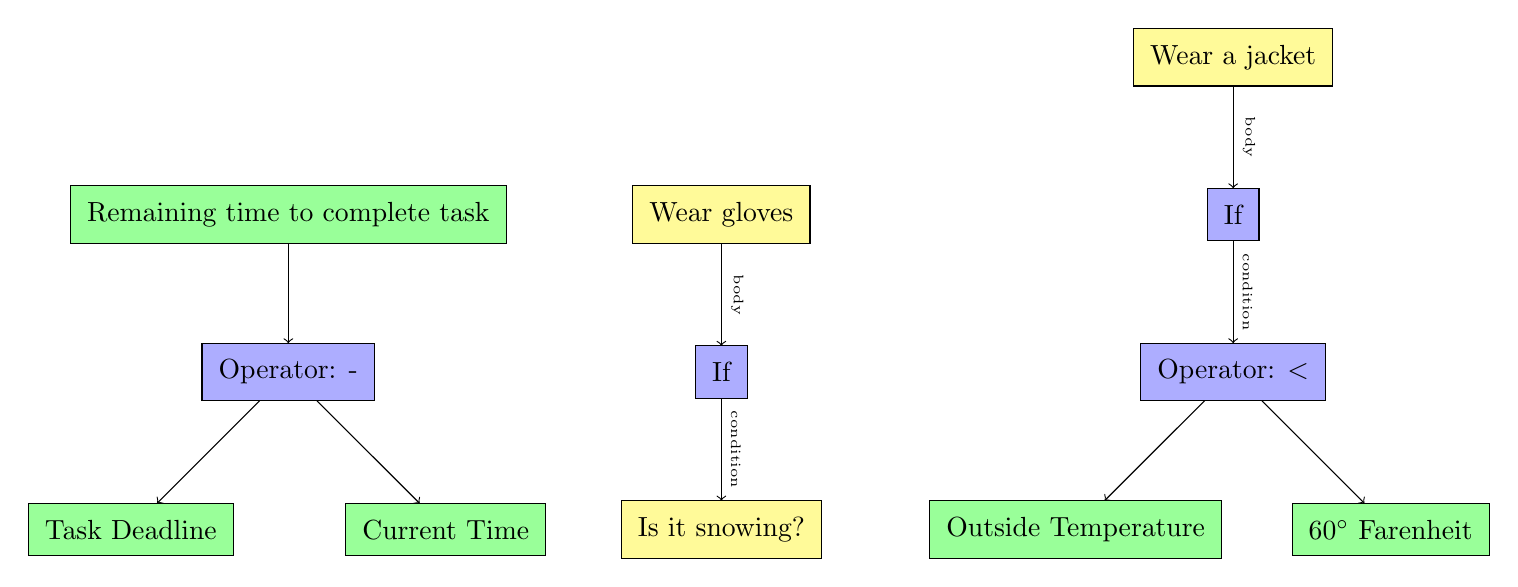
\begin{tikzpicture}
		
		\tikzstyle{operation} = [shape=rectangle, draw, outer sep=0,inner  sep=6,minimum size=15, fill = blue!32]
		\tikzstyle{value} = [shape=rectangle, draw, outer sep=0,inner  sep=6,minimum size=15, fill = green!40]
		\tikzstyle{logic} = [shape=rectangle, draw, outer sep=0,inner  sep=6,minimum size=15, fill = yellow!40]
		\tikzstyle{function} = [shape=rectangle, draw, outer sep=0,inner  sep=6,minimum size=15, fill = red!40]
		\tikzstyle{con} = [thick,->]
		
		\node[value] (TimeLeft) at (4,4) {Remaining time to complete task};
		\node[operation] (Subtract) at (4,2) {Operator: -};
		\node[value] (Deadline) at (2,0) {Task Deadline};
		\node[value] (CurrentTime) at (6,0) {Current Time};
		
		\draw[->](TimeLeft) -> (Subtract) ;	
		\draw[->](Subtract) -> (Deadline) ;	
		\draw[->](Subtract) -> (CurrentTime) ;	
		
		
		\node[operation] (Subtract) at (9.5,2) {If};
		\node[logic] (Deadline) at (9.5,0) {Is it snowing?};
		\node[logic] (CurrentTime) at (9.5,4) {Wear gloves};
		
		\draw[->](Subtract) -> (Deadline) node[midway,sloped,above] {\tiny condition};	
		\draw[->](CurrentTime) -> (Subtract) node[midway,sloped,above] {\tiny body} ;	
		
		
		\node[logic] (Jacket) at (16,6) {Wear a jacket};
		\node[operation] (TimeLeft) at (16,4) {If};
		\node[operation] (Subtract) at (16,2) {Operator: $<$};
		\node[value] (Deadline) at (14,0) {Outside Temperature};
		\node[value] (CurrentTime) at (18,0) {60$^{\circ}$ Farenheit};
		
		\draw[->](Jacket) -> (TimeLeft) node[midway,sloped,above] {\tiny body} ;	
		\draw[->](TimeLeft) -> (Subtract)  node[midway,sloped,above] {\tiny condition} ;	
		\draw[->](Subtract) -> (Deadline) ;	
		\draw[->](Subtract) -> (CurrentTime) ;	
		
		\end{tikzpicture}
		
		\caption{Three abstract trees that each represent a simple decision using numerical and/or binary categorical information}
		
	\end{figure}    
	
	
	Neural networks have been used for decades to solve a wide variety of machine learning tasks without the need for explicit programming of the solutions to be done by humans. Typically the networks only make use of arithmetic computation, meaning that logical operations are not incorportated into the models. This hasn't been done because there is no clear method by which logical information (TRUE/FALSE) should be converted to numerical information, and vice versa. In Computer Science, True and False are generally represented as 1 and 0, respectively, whereas in Mathematics, they are often represented as -1 and 1 \textcolor{red}{Which specific fields of Math and Compsci?}. Our research aims to construct a neural network which effectively combines logical and arithmetic computation, and apply this network to a problem which demostrates it's ability to perform symbolic reasoning.
	\textcolor{red} {- old background} \\
	
	\begin{enumerate}
		\item What is symbolic computation?
		
		A symbolic computation is a calculation performed with symbolic representations of values and operations. A simple example would be the expression $(x + 1)(x - 1)$ which would evaluate to $x^2 - 1$, rather than to some numerical result.
		
		\item What is calculation?
		
		A calculation is a process by which one or more inputs is transformed into one or more results. One may calculate that the product of 5 and 4 is 20.
		
		\item What is meant by a computational class? \textcolor{red}{- do you mean complexity class?}
		
		
	\end{enumerate}
	
	Code for each subsection of this document can be found at \href{https://github.com/DariusBxsci/NeuralNetworkResearch/tree/master/NeuralNets}{NeuralNetworkResearch}. 
	
	\subsection{What is an Artificial Neural Network?}
	
		An Artificial Neural Network is a computational system of interconnected units, called neurons, such that signals may pass indirectly from a group of neurons, called input neurons, to another group of neurons, called output neurons. The connections between neurons often involve weights, which modify the value of the signal before passing it to the next neuron. Each weight can be adjusted (either manually or via some training algorithm) such that possible input values will yield corresponding desired output values.
	
	\section{Methods}
	
	\subsection{Network Construction}
	
	Figure \ref{fig:sig-neuron} illustrates a neuron that receives three ordered inputs. 
	
	
	\begin{figure}[!htb]
		
		\centering
		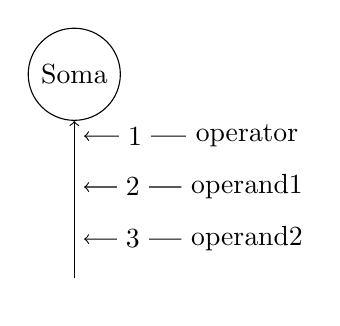
\begin{tikzpicture}
		
		
		\node[circle, draw=black] (soma) {Soma};
		\node[below= 2cm of soma] (dendrite) {};
		
		\begin{scope}[node distance=1mm and 10mm]
		\node[below right = of soma] (operator) {operator};
		\node[below = of operator] (operand1) {operand1};
		\node[below = of operand1] (operand2) {operand2};
		\end{scope}
		
		
		\draw[->] (dendrite) -> (soma);
		
		
		%nodes along dendrite
		\node (operator'dendrite) at (intersection of operator--soma|-operator and dendrite--soma){};
		
		\node (operand1'dendrite) at (intersection of operand1--soma|-operand1 and dendrite--soma){};
		
		\node (operand2'dendrite) at (intersection of operand2--soma|-operand2 and dendrite--soma){};
		
		
		\draw[->] (operator) -- (operator'dendrite) node[midway, fill=white] {1};
		\draw[->] (operand1) -- (operand1'dendrite) node[midway, fill=white] {2};
		\draw[->] (operand2) -- (operand2'dendrite) node[midway, fill=white] {3};
		
		\end{tikzpicture}
		\caption{Single neuron receiving ordered intputs. \label{fig:sig-neuron}}
	\end{figure}
	
	
	While this model is suitable for biological networks of neurons, a neural network in the computational sense would look more like an abstract syntax tree. In the following diagram, a network of operators and operands form a tree-like structure in which elements at lower levels represent values to manipulate which at higher levels interact with each other through arithmetic operations to produce a result. Any computation which involves a combination of operations on one or more values can be represented in this structure, such as logical or arithmetic operations.
	
	
	\begin{figure}[!htb]
		\centering
		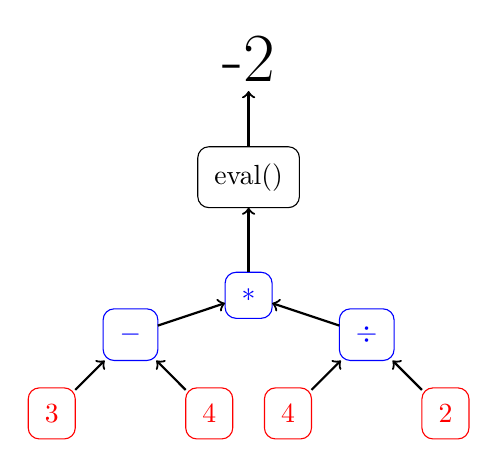
\begin{tikzpicture}
		
		\tikzstyle{bordered} = [shape=rectangle, rounded corners, draw, outer sep=0,inner sep=6,minimum size=15]
		\tikzstyle{con} = [thick,->]
		\tikzstyle{message} = [shape=rectangle, thick, minimum width=2cm]
		
		\node [bordered,red] (v1) at (1.5,8) {3};
		\node [bordered,red] (v5) at (3.5,8) {4};
		\node [bordered,red] (v4) at (4.5,8) {4};
		\node [bordered,red] (v3) at (6.5,8) {2};
		
		\node [bordered,blue] (v6) at (5.5,9) {$\div$};
		\node [bordered,blue] (v2) at (2.5,9) {$-$};
		
		\node [bordered,blue] (v7) at (4,9.5) {$*$};
		
		\node [bordered,black] (v8) at (4,11) {eval()};
		
		\node [black] (v9) at (4,12.5) {\Huge -2};
		
		\draw [con] (v1) edge (v2);
		\draw [con] (v3) edge (v6);
		\draw [con] (v4) edge (v6);
		\draw [con] (v5) edge (v2);
		
		\draw [con] (v2) edge (v7);
		\draw [con] (v6) edge (v7);
		
		\draw [con] (v7) edge (v8);
		
		\draw [con] (v8) edge (v9);
		
		
		\end{tikzpicture}
		\caption{An Abstract Syntax Tree of arithmetic operations.} 
	\end{figure}
	
	\begin{figure}[!htb]
		\centering
		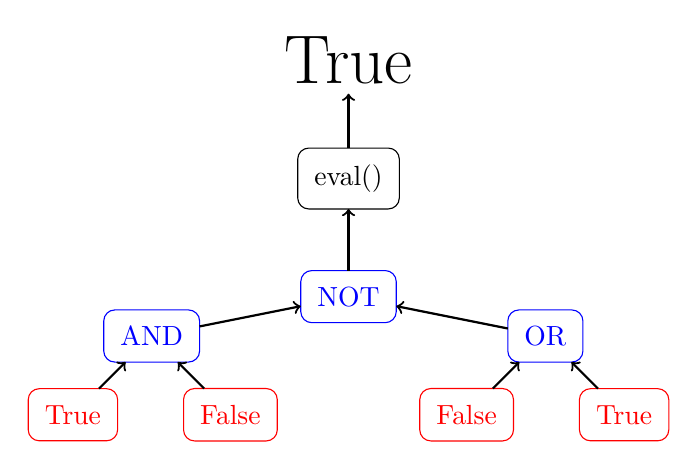
\begin{tikzpicture}
		
		\tikzstyle{bordered} = [shape=rectangle, rounded corners, draw, outer sep=0,inner    sep=6,minimum size=15]
		\tikzstyle{con} = [thick,->]
		\tikzstyle{message} = [shape=rectangle, thick, minimum width=2cm]
		
		\node [bordered,red] (v1) at (0.5,8) {True};
		\node [bordered,red] (v5) at (2.5,8) {False};
		\node [bordered,red] (v4) at (5.5,8) {False};
		\node [bordered,red] (v3) at (7.5,8) {True};
		
		\node [bordered,blue] (v6) at (6.5,9) {OR};
		\node [bordered,blue] (v2) at (1.5,9) {AND};
		
		\node [bordered,blue] (v7) at (4,9.5) {NOT};
		
		\node [bordered,black] (v8) at (4,11) {eval()};
		
		\node [black] (v9) at (4,12.5) {\Huge True};
		
		\draw [con] (v1) edge (v2);
		\draw [con] (v3) edge (v6);
		\draw [con] (v4) edge (v6);
		\draw [con] (v5) edge (v2);
		
		\draw [con] (v2) edge (v7);
		\draw [con] (v6) edge (v7);
		
		\draw [con] (v7) edge (v8);
		
		\draw [con] (v8) edge (v9);sudo apt-get install --no-install-recommends texlive-latex-extra
		
		
		\end{tikzpicture}
		\caption{An Abstract Syntax Tree of logical operations.} 
	\end{figure}
	
	\subsection{Using each arithmetic operator with a logical operand} 
	{\it Code that corresponds with this section can be found in NeuralNetwork\_5.py}
	
	Syntax trees such as the ones shown above work perfectly, since each contain exclusively arithmetic or logical computations. In the trees shown below, however, the two computation classes are combined through multiplication and addition. The tree's results depend entirely on how we choose to evaluate $2 * True$ and $2 + True$.
	
	\newpage	
	
	\begin{figure}[!htb]
		\centering
		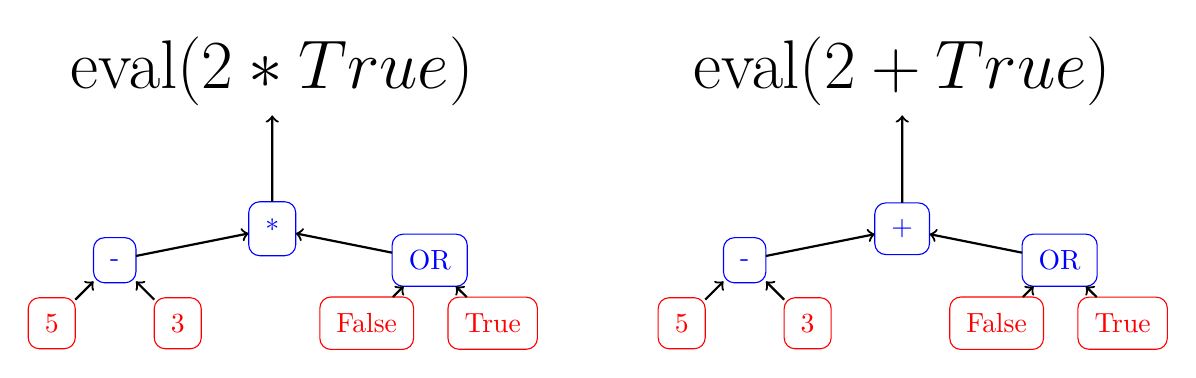
\begin{tikzpicture}[scale=0.8]
		
		\tikzstyle{bordered} = [shape=rectangle, rounded corners, draw, outer sep=0,inner    sep=6,minimum size=15]
		\tikzstyle{con} = [thick,->]
		\tikzstyle{message} = [shape=rectangle, thick, minimum width=2cm]
		
		\node [bordered,red] (v1) at (0.5,8) {5};
		\node [bordered,red] (v5) at (2.5,8) {3};
		\node [bordered,red] (v4) at (5.5,8) {False};
		\node [bordered,red] (v3) at (7.5,8) {True};
		
		\node [bordered,blue] (v6) at (6.5,9) {OR};
		\node [bordered,blue] (v2) at (1.5,9) {-};
		
		\node [bordered,blue] (v7) at (4,9.5) {*};
		
		
		\node [black] (v9) at (4,12) {\Huge eval($2 * True$)};
		
		\draw [con] (v1) edge (v2);
		\draw [con] (v3) edge (v6);
		\draw [con] (v4) edge (v6);
		\draw [con] (v5) edge (v2);
		
		\draw [con] (v2) edge (v7);
		\draw [con] (v6) edge (v7);
		
		\draw [con] (v7) edge (v9);
		
		
		\node [bordered,red] (vv1) at (10.5,8) {5};
		\node [bordered,red] (vv5) at (12.5,8) {3};
		\node [bordered,red] (vv4) at (15.5,8) {False};
		\node [bordered,red] (vv3) at (17.5,8) {True};
		
		\node [bordered,blue] (vv6) at (16.5,9) {OR};
		\node [bordered,blue] (vv2) at (11.5,9) {-};
		
		\node [bordered,blue] (vv7) at (14,9.5) {+};
		
		\node [black] (vv9) at (14,12) {\Huge eval($2 + True$)};
		
		\draw [con] (vv1) edge (vv2);
		\draw [con] (vv3) edge (vv6);
		\draw [con] (vv4) edge (vv6);
		\draw [con] (vv5) edge (vv2);
		
		\draw [con] (vv2) edge (vv7);
		\draw [con] (vv6) edge (vv7);
		
		\draw [con] (vv7) edge (vv9);
		
		\end{tikzpicture}
		\caption{Abstract Syntax Trees of logical and arithmetic operations.} 
	\end{figure}
	
	An error would be the result if the two expressions were to be evaluated since $True$ and $False$ are not numerical values so they aren't compatible with numerical operations like $*$ and $+$. Now the question arises, {\it How can logical symbols be converted into numerical values?} In the context of Computer Science and Programming, one may represent $False$ as $0$ and $True$ as $1$. In the case of multiplication, this format would cause $eval()$ to yield $0$ if one of the operands is $False$ and whatever the other operand is if one is $True$. Let us now model a real-world situation in which logical and arithmetic computation are both necessary for a result.
	
	\begin{figure}[H]
		
		\begin{subfigure}{1.0\textwidth}
			\centering
			
			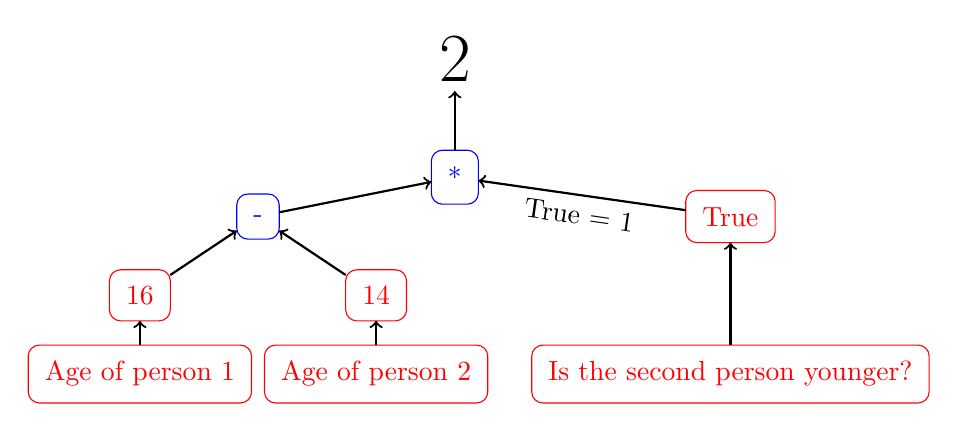
\begin{tikzpicture}
			
			\tikzstyle{bordered} = [shape=rectangle, rounded corners, draw, outer sep=0,inner    sep=6,minimum size=15]
			\tikzstyle{con} = [thick,->]
			\tikzstyle{message} = [shape=rectangle, thick, minimum width=2cm]
			
			\node [bordered,red] (vm1) at (0,6.5) {Age of person 1};
			\node [bordered,red] (vm5) at (3,6.5) {Age of person 2};
			\node [bordered,red] (v1) at (0,7.5) {16};
			\node [bordered,red] (v5) at (3,7.5) {14};
			
			\node [bordered,red] (v4) at (7.5,6.5) {Is the second person younger?};
			\node [bordered,red] (v3) at (7.5,8.5) {True};
			
			\node [bordered,blue] (v2) at (1.5,8.5) {-};
			
			\node [bordered,blue] (v7) at (4,9) {*};
			
			
			\node [black] (v9) at (4,10.5) {\Huge 2};
			
			\draw [con] (vm1) edge (v1);
			\draw [con] (vm5) edge (v5);	
			
			\draw [con] (v1) edge (v2);
			\draw [con] (v4) edge (v3);
			\draw [con] (v5) edge (v2);
			
			\draw [con] (v3) edge node[sloped, below] {True = 1}  (v7);
			
			\draw [con] (v2) edge(v7);
			
			\draw [con] (v7) edge (v9);
			
			\end{tikzpicture}
			
			\caption{First sibling is younger}    
			
		\end{subfigure}
		
		\begin{subfigure}{1.0\textwidth}
			\centering
			
			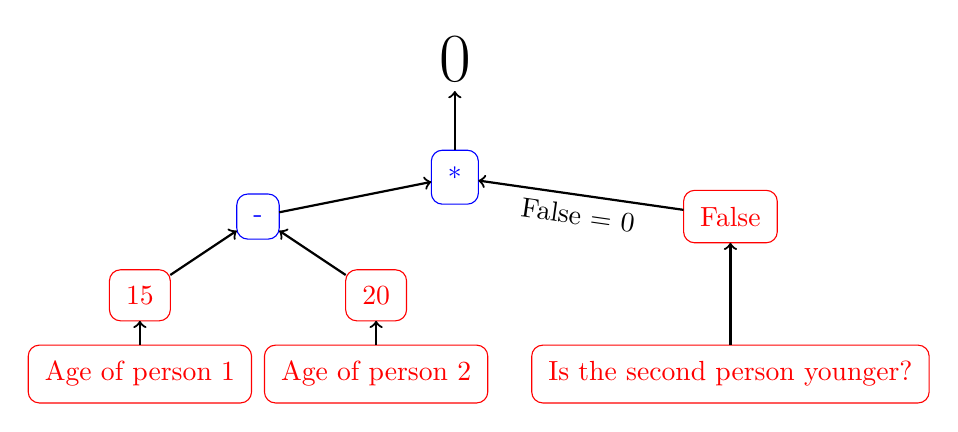
\begin{tikzpicture}
			
			\tikzstyle{bordered} = [shape=rectangle, rounded corners, draw, outer sep=0,inner    sep=6,minimum size=15]
			\tikzstyle{con} = [thick,->]
			\tikzstyle{message} = [shape=rectangle, thick, minimum width=2cm]
			
			\node [bordered,red] (vm1) at (0,6.5) {Age of person 1};
			\node [bordered,red] (vm5) at (3,6.5) {Age of person 2};
			\node [bordered,red] (v1) at (0,7.5) {15};
			\node [bordered,red] (v5) at (3,7.5) {20};
			
			\node [bordered,red] (v4) at (7.5,6.5) {Is the second person younger?};
			\node [bordered,red] (v3) at (7.5,8.5) {False};
			
			\node [bordered,blue] (v2) at (1.5,8.5) {-};
			
			\node [bordered,blue] (v7) at (4,9) {*};
			
			
			\node [black] (v9) at (4,10.5) {\Huge 0};
			
			\draw [con] (vm1) edge (v1);
			\draw [con] (vm5) edge (v5);	
			
			\draw [con] (v1) edge (v2);
			\draw [con] (v4) edge (v3);
			\draw [con] (v5) edge (v2);
			
			\draw [con] (v3) edge node[sloped, below] {False = 0}  (v7);
			
			\draw [con] (v2) edge(v7);
			
			\draw [con] (v7) edge (v9);
			
			\end{tikzpicture}  
			
			\caption{Second sibling is younger}
			
		\end{subfigure}
		
		\caption{A syntax tree which models how many years one person is older than another, using a combination of Arithmetic and Logical computation.} 
	\end{figure}
	
	
	In the above trees, logical and numerical information are effectively combined to produce an output. If only numerical information were used (i.e. the ages of the two people), only the difference of the two numbers would be calculated, yielding $-5$ in the second case. However, a person cannot be a negative number of years older than another, so $0$ would be a more appropriate result. The above trees solve this problem by requiring the user to give a boolean value representing whether or not the second person is younger than the first, then the $True/False$ value is converted into a number according to previously defined policy and multiplied with the difference of the two ages. \\
	
	We have just successfully formulated a method by which logical symbols and numbers can be combined through the multiplication operator, but how would the two be combined through the subtraction, division, and addition operators? \\
	
	The process of multiplication can be broken down into a series of repeated additions. For example, $4 * 3$ is the same as $4 + 4 + 4$. Therefor, the expression $4 * True$ can be broken down into $True + True + True + True$. Let us add $True$ to this expression and get $True + True + True + True + True$, and simplify it to just $5 * True$ (by the distributive property of multiplication), which by our multiplication rule would evaluate to $5$. By this logic, adding $True$ to a value is equivalent to adding $1$, and adding $False$ is equivalent to adding $0$. We can extend this to subtraction, so that subtracting $True$ subtracts $1$ and $False$ subtracts $0$ \\
	
	The division and multiplication operators are inverse operations. In other words, if a number is divided by number, $x$, multiplying the result by $x$ would yield the original number. Naturally, this relationship should remain when using logical operands. However, this poses a major problem since if a value is multiplied by $False$, the output will be $0$, and there is no number that $False$ can be converted into such that dividing $0$ by it will yield the initial value (if the initial value is not $0$).
	\textcolor{red}{- How can/should this problem be reconciled?} \\
	
	\subsection{An alternative solution}
	
	In the previous subsection, we attempted to solve the problem of combining logical and numerical symols by converting $True$ into $1$ and $False$ into $2$. In doing this, we noticed that the multiplication operator could be used with a logical symbol to either propogate or to destroy a numerical signal. On the other hand, we were not able to put the addition, subtraction, and division operators to meaningful use, as we were with multiplication. From these results, it should be clear that an alternative solution is necessary. To discover this solution, we will examine a few situations where the two brands of computation are necessary, and formulate how the two can be combined into one family of computations. 
	
	(a tree which models a situation where logical and numerical information need to be combined via some operator) \textcolor{red}{- What sort of situation REQUIRES this? (TemperatureTree is a possibility)}
	
	It is unclear how the two should be combined such that the meaning behind each value is retained. In the above situation... (describe how one would combine the two in the above situation to yield the correct output). \\ \\
	
	\textcolor{red}{Ideas for solving the problem of combining the two forms of information:}
	
	\begin{enumerate}
		
		\item The simplest solution would be to simply convert all information into one type, rather than having them be separate. The issue with this that the converted information may lose it's representational meaning.
		
		\item Another solution would be to store all information as a tuple with a numerical element and a logical element. Numerical operations would exclusively act on numbers and logical operations on logical symbols.
		
		\item Some new data structure could be made which exists as a postion in space, where one dimension describes logical state and the other describes numerical state. Similar to points on a cartesian plane, except the 'x' axis would be True/False, and the 'y' axis would be a numerical value. Operations could be performed on this object as transformations in the same way they could be done to points on an xy plane. This solution could be advantageous in the long run since any new data type can be added to the data structure by adding a new dimension for it and tranforming points in operations in the same way.
		
	\end{enumerate}
	
	
	\subsection{Combining computation through conditional statements}
	% https://en.wikipedia.org/wiki/Abstract_syntax_tree#/media/File:Abstract_syntax_tree_for_Euclidean_algorithm.svg
	
	Conditional statements, such as $if$ and $while$ may be used to combine categorical and numerical computation. Each conditional statement accepts an input expression, and has a body which is defined before runtime. If the input expression evaluates to $True$, then the statement will execute whatever is in the body. The body may contain computations of any kind, including numerical. In the following examples, conditional statements are used to execute some numerical computations depending on the result of some categorical computations.
	
	\newpage	
	
	\begin{figure}
		\centering
		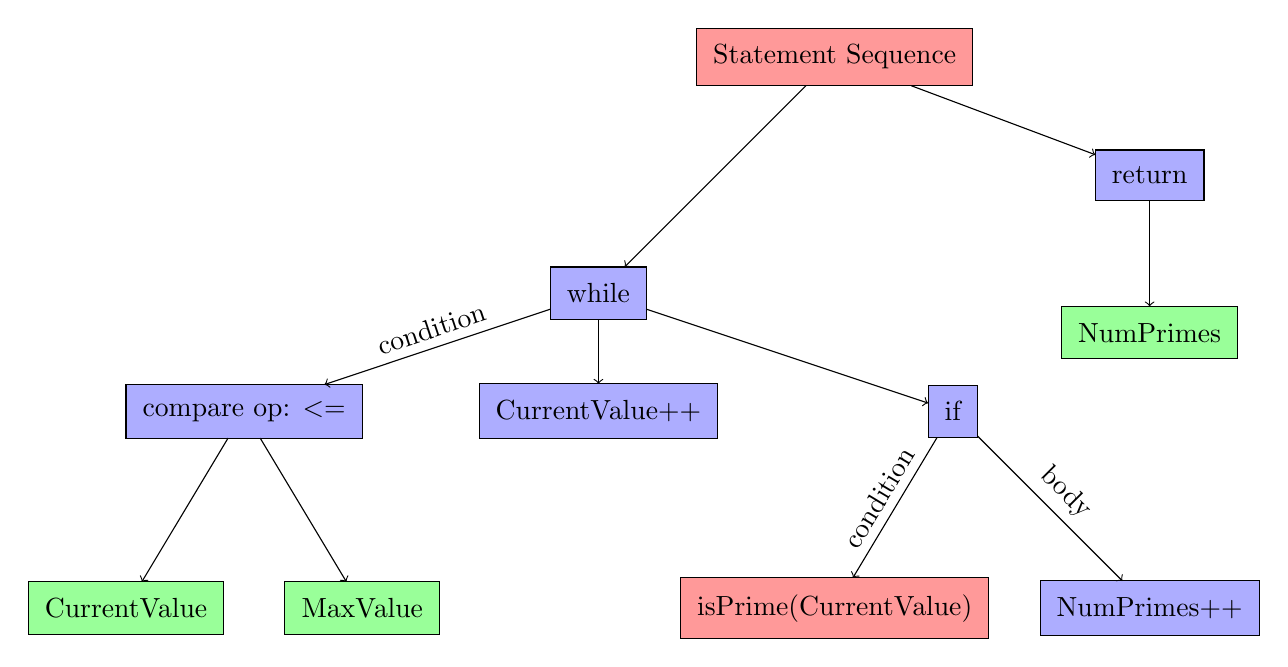
\begin{tikzpicture}
		
		\tikzstyle{operation} = [shape=rectangle, draw, outer sep=0,inner  sep=6,minimum size=15, fill = blue!32]
		\tikzstyle{value} = [shape=rectangle, draw, outer sep=0,inner  sep=6,minimum size=15, fill = green!40]
		\tikzstyle{function} = [shape=rectangle, draw, outer sep=0,inner  sep=6,minimum size=15, fill = red!40]
		\tikzstyle{con} = [thick,->]
		
		\node[function] (StatementSequence) at (9,7) {Statement Sequence};
		
		\node[operation] (return) at (13,5.5) {return};
		\node[value] (returnVal) at (13,3.5) {NumPrimes};
		
		\draw[->](StatementSequence) -> (return) ;	
		\draw[->](return) -> (returnVal) ;	
		
		\node[operation] (while) at (6,4) {while};
		\node[value] (CurrentValue) at (0,0) {CurrentValue};
		\node[value] (MaxValue) at (3,0) {MaxValue};
		\node[operation] (lessThan) at (1.5,2.5) {compare op: $<=$};
		
		\draw[->](StatementSequence) -> (while) ;	
		\draw[->](while) -> (lessThan) node[midway,sloped,above] {condition} ;	
		\draw[->](lessThan) -> (MaxValue) ;	
		\draw[->](lessThan) -> (CurrentValue) ;	
		
		\node[operation] (incrementCurr) at (6,2.5) {CurrentValue++};
		\draw[->](while) -> (incrementCurr) ;	
		
		\node[operation] (branch) at (10.5,2.5) {if};
		\node[function] (isPrime) at (9,0) {isPrime(CurrentValue)};
		\node[operation] (incrementPrime) at (13,0) {NumPrimes++};
		
		\draw[->](while) -> (branch) ;
		\draw[->](branch) -> (isPrime)  node[midway,sloped,above] {condition};		
		\draw[->](branch) -> (incrementPrime)  node[midway,sloped,above] {body};	
		
		\end{tikzpicture}
		
		\caption{A syntax tree that defines a procedure for counting the number of primes up to a certain value. The procedure begins with NumPrimes and CurrentValue set to $0$, and MaxValue set to the highest value to check for prime status. isPrime is a function that returns $True$ if the input value is a prime number, and $False$ if it isn't. \\} 
		
	\end{figure}
	
	In the above example, a $while$ conditional statement repeatedly executes it's body as long as $CurrentValue <= MaxValue$ evaluates to $True$ (meaning that CurrentValue is either less than or equal to the MaxValue). In $while$'s body, the $CurrentValue$ is incremented by one then $NumPrimes$ is incremented if the $CurrentValue$ is a prime number. 
	
	
	
	\subsection{The relationship between numerical and categorical information}
	
	Numerical information consists of numerical values, such that there exists infinitely many numerical values between two numbers. This property makes numerical information continuous. In contrast, categorical information involves individual values out of a set of either finite or infinite possible values. Categorical information are discrete, however, so there exists a finite number of categories between any two categories.
	
	
	\subsection{Routing categorical information through a neural network}
	
	Information is represented in one of two ways, numerical or categorical. Numerical values give us the ability to identify the distance between two values, and to have an infinite number of possible values to work with. Categorical values allow us to express information where a specific value to represent the distance between two categories isn't appropriate. We can also express more vague values using categories, without the need for specific numerical values.
	We can express the speed that an object is moving using either numerical or categorical values. For instance, we may say that an object is moving at exactly 50 miles per hour, or we can simply say that the object is moving 'fast'. In the following figures, we will examine how to convert between the two types.
	
	\begin{figure}[!htb]
		
		\centering
		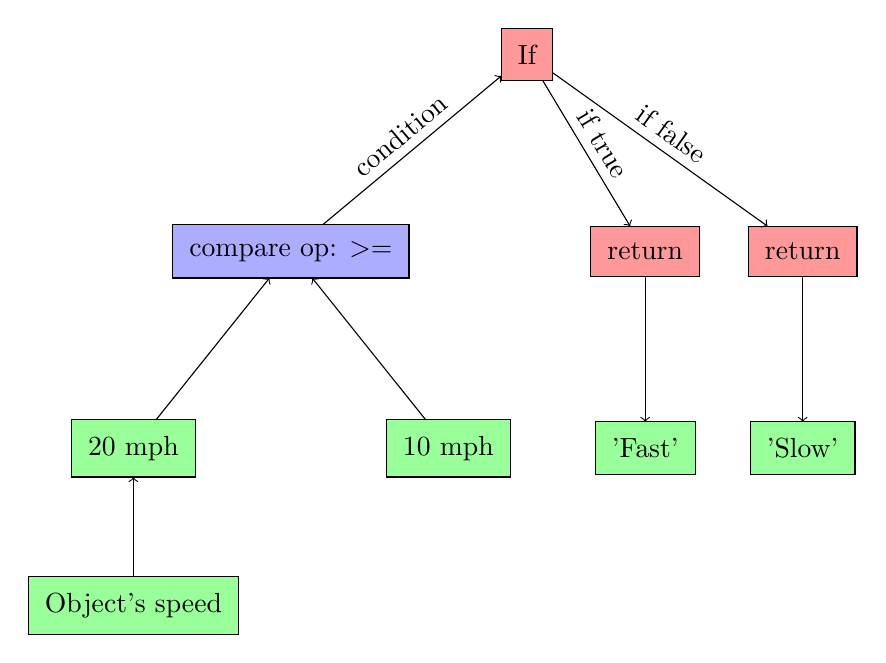
\begin{tikzpicture}
		
		\tikzstyle{operation} = [shape=rectangle, draw, outer sep=0,inner  sep=6,minimum size=15, fill = blue!32]
		\tikzstyle{value} = [shape=rectangle, draw, outer sep=0,inner  sep=6,minimum size=15, fill = green!40]
		\tikzstyle{function} = [shape=rectangle, draw, outer sep=0,inner  sep=6,minimum size=15, fill = red!40]
		\tikzstyle{con} = [thick,->]
		
		\node[value] (ObjectSpeed) at (0,-2) {Object's speed};
		\node[value] (Speed) at (0,0) {20 mph};
		
		\node[operation] (greaterThan) at (2,2.5) {compare op: $>=$};
		
		\node[value] (SpeedComp) at (4,0) {10 mph};
		
		\node[function] (If) at (5,5) {If};
		
		\node[function] (Return1) at (6.5,2.5) {return};
		\node[value] (Fast) at (6.5,0) {'Fast'};
		
		\node[function] (Return2) at (8.5,2.5) {return};
		\node[value] (Slow) at (8.5,0) {'Slow'};
		
		\draw[->](ObjectSpeed) -> (Speed)  node[midway,sloped,above] {};
		
		\draw[->](Speed) -> (greaterThan)  node[midway,sloped,above] {};
		\draw[->](SpeedComp) -> (greaterThan)  node[midway,sloped,above] {};	
		
		\draw[->](greaterThan) -> (If)  node[midway,sloped,above] {condition};	
		
		\draw[->](If) -> (Return1)  node[midway,sloped,above] {if true};	
		\draw[->](If) -> (Return2)  node[midway,sloped,above] {if false};	
		
		\draw[->](Return1) -> (Fast)  node[midway,sloped,above] {};	
		\draw[->](Return2) -> (Slow)  node[midway,sloped,above] {};	
		
		\end{tikzpicture}
		
		\caption{A syntax tree that defines a procedure for converting categorical representations to numerical ones. In this case, a threshold of 10mph is defined to detirmine whether a numerical definition of the speed of an object is 'Fast' or 'Slow' depending on whether or not the object's speed is above or below the threshold.} 
		
	\end{figure}
	
	The threshold used in the above procedure is arbitrary, and can be defined differently in different networks. \textcolor{red} {This idea can be used to create a network where this threshold is optimized through gradient descent (similarly to the ReLu activation function with a variable bias)}
	
	\subsection{Using conditional expressions to vary computations of neurons}
	
	Consider a simple network with two input neurons, two corresponding weights, and a single output neuron.
	
	\begin{figure}[!htb]
		
		\centering
		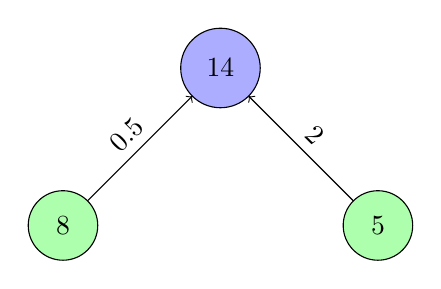
\begin{tikzpicture}
		
		\tikzstyle{input} = [shape=circle, draw, outer sep=0,inner  sep=6,minimum size=15, fill = green!32]
		\tikzstyle{output} = [shape=circle, draw, outer sep=0,inner  sep=6,minimum size=15, fill = blue!32]
		\tikzstyle{weight} = [thick,midway,sloped,above,->]
		
		\node[input] (i1) at (0,0) {8};
		\node[input] (i2) at (4,0) {5};
		
		\node[output] (o1) at (2,2) {14};
		
		\draw[->](i1) -> (o1) node[weight] {0.5};
		\draw[->](i2) -> (o1) node[weight] {2};
		
		\end{tikzpicture}
		
		\caption{A simple feed-forward neural network with two inputs and one output.}
		
	\end{figure}
	
	\newpage
	
	In the above network, the output neuron's value is calculated as a weighted sum of the inputs. While this algorithm is widely used in feed-forward neural networks, it assumes that the desired output value's relationship to it's inputs can be modelled by a weighted sum of the inputs.  \\
	
	Suppose we wanted to construct a network that returns the number of times older one person is than another. Given the inputs of 24 and 8, the output would be 3 since a 24-year-old is 3 times older than an 8-year-old. However, this relationship cannot be expressed through a weighted sum, since no weighted sum of two variables will always equal the quotient of the two variables. To deal with this problem, we will introduce a 'router' that will allow for more than just a weighted sum to define the output.
	
	\begin{figure}[!htb]
		
		\centering
		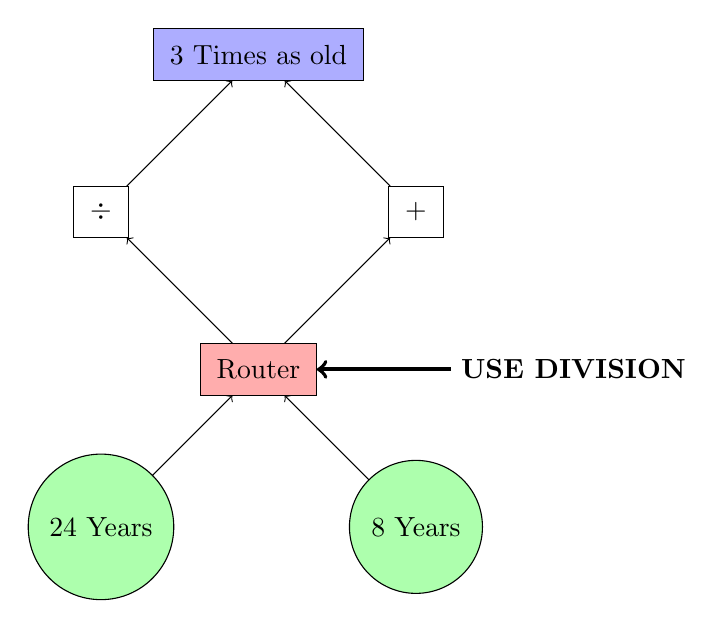
\begin{tikzpicture}
		
		\tikzstyle{input} = [shape=circle, draw, outer sep=0,inner  sep=6,minimum size=15, fill = green!32]
		\tikzstyle{output} = [shape=rectangle, draw, outer sep=0,inner  sep=6,minimum size=15, fill = blue!32]
		\tikzstyle{router} = [shape=rectangle, draw, outer sep=0,inner  sep=6,minimum size=15, fill = red!32]
		\tikzstyle{op} = [shape=rectangle, draw, outer sep=0,inner  sep=6,minimum size=18]
		\tikzstyle{weight} = [thick,midway,sloped,above,->]
		
		\node[input] (i1) at (0,0) {24 Years};
		\node[input] (i2) at (4,0) {8 Years};
		
		\node[font=\bf] (dum) at (6,2) {USE DIVISION};
		\node[router] (r) at (2,2) {Router};
		
		\node[op] (op1) at (0,4) {$\div$};
		\node[op] (op2) at (4,4) {$+$};
		
		\node[output] (o1) at (2,6) {3 Times as old};
		
		\draw[->](i1) -> (r) node[weight] {};
		\draw[->](i2) -> (r) node[weight] {};
		
		\draw[->,line width=0.5mm](dum) -> (r) {};
		
		\draw[->](r) -> (op1) node[weight] {};
		\draw[->](r) -> (op2) node[weight] {};
		
		\draw[->](op1) -> (o1) node[weight] {};
		\draw[->](op2) -> (o1) node[weight] {};
		
		
		
		\end{tikzpicture}
		
		\caption{A network which yields the number of times a person is older than another.}
		
	\end{figure}
	
	The 'Router' represents some function which decides which computational class should be used to compute the output. In the above network, we instructed the router to operate on input values using division, since that was how we detirmined that the task could be solved. \\
	
	Of course, instructing the router as to which computation it should use in each input case defeats it's purpose. Instead, we may use conditional statements to determine which computation will be used. This allows us to construct networks which perform different classes of computation depending on the situation. One such network is shown below.
	
	\newpage
	
	\begin{figure}
		
		\centering
		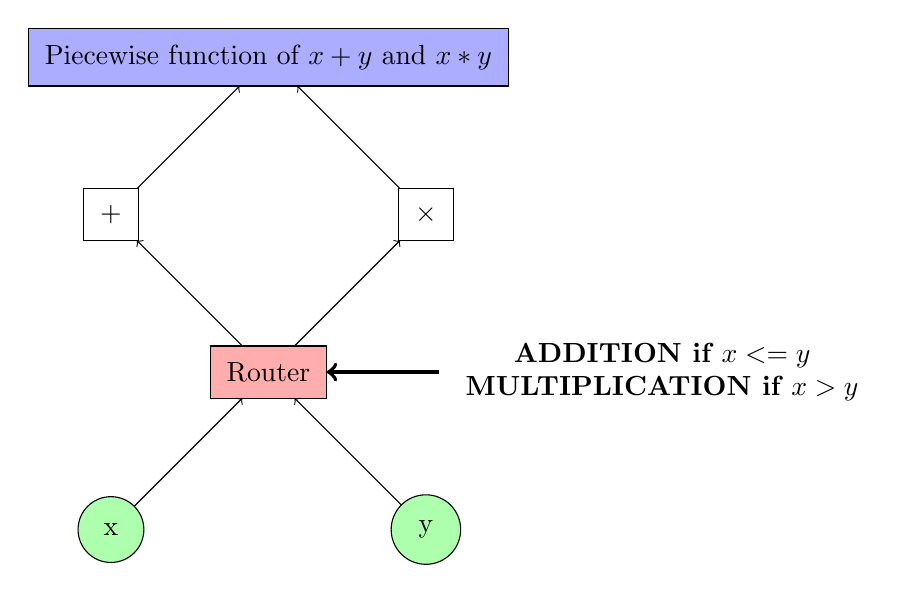
\begin{tikzpicture}[shift={(current page.center)}]
		
		\tikzstyle{input} = [shape=circle, draw, outer sep=0,inner  sep=6,minimum size=15, fill = green!32]
		\tikzstyle{output} = [shape=rectangle, draw, outer sep=0,inner  sep=6,minimum size=15, fill = blue!32]
		\tikzstyle{router} = [shape=rectangle, draw, outer sep=0,inner  sep=6,minimum size=15, fill = red!32]
		\tikzstyle{op} = [shape=rectangle, draw, outer sep=0,inner  sep=6,minimum size=18]
		\tikzstyle{weight} = [thick,midway,sloped,above,->]
		
		\node[input] (i1) at (0,0) {x};
		\node[input] (i2) at (4,0) {y};
		
		\node[font=\bf] (dum) at (7,2) {
			\begin{tabular}{cc}
			ADDITION if $x <= y$ \\
			MULTIPLICATION if $x > y$
			\end{tabular}
		};
		
		\node[router] (r) at (2,2) {Router};
		
		\node[op] (op1) at (0,4) {$+$};
		\node[op] (op2) at (4,4) {$\times$};
		
		\node[output] (o1) at (2,6) {Piecewise function of $x + y$ and $x * y$};
		
		\draw[->](i1) -> (r) node[weight] {};
		\draw[->](i2) -> (r) node[weight] {};
		
		\draw[->,line width=0.5mm, loop above](dum) -> (r) {};
		
		\draw[->](r) -> (op1) node[weight] {};
		\draw[->](r) -> (op2) node[weight] {};
		
		\draw[->](op1) -> (o1) node[weight] {};
		\draw[->](op2) -> (o1) node[weight] {};
		
		
		\end{tikzpicture}
		
		\caption{A simple piecewise function modeled by a router network}
		
	\end{figure}
	
	The above network models a piecewise function of the expressions $x + y$ and $x * y$, where $x$ and $y$ are inputs. A typical neural network which uses weighted sums and sigmoid activation functions would require many neurons and considerable training to model this function.
	
	\subsection{Are Neural Networks Turing Complete?}

		For something to be Turing complete, it must be able to do anything that a Turing Machine can do. All that a Turing Machine can do is read each cell in a tape of 1's and 0's, write to each cell, and go to each cell. For a Turing Machine to be able to compute anything (given an infinite amount of time), it must use a tape that may have infinite length. 
		
		To decide whether or not a Neural Network is Turing complete, we need to imagine a simple Turing Machine. Suppose we have a turing machine which switches two numbers, such that the output is the reverse of the input. To do this, the first number must be stored in a buffer cell, the first cell should be set to the value of the second cell, and the second cell should be set to the value of the buffer. Notice that the contents of the tape in this machine may be any integer value, rather than just 1 or 0. 
		
		\newpage
		\begin{figure}
			
			\centering
			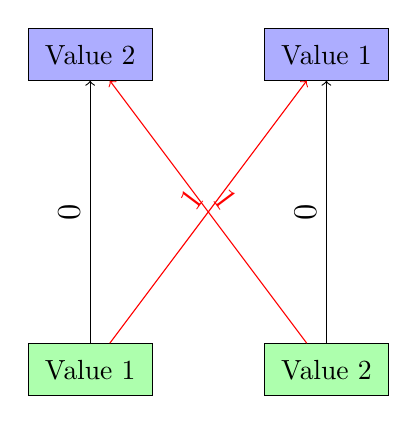
\begin{tikzpicture}
			
				\tikzstyle{input} = [shape=rectangle, draw, outer sep=0,inner  sep=6,minimum size=15, fill = green!32]
				\tikzstyle{output} = [shape=rectangle, draw, outer sep=0,inner  sep=6,minimum size=15, fill = blue!32]
				\tikzstyle{weight} = [thick,midway,sloped,above,->]
				
				\node[input] (i1) at (0,0) {Value 1};
				\node[input] (i2) at (3,0) {Value 2};
				
				\node[output] (o1) at (0,4) {Value 2};
				\node[output] (o2) at (3,4) {Value 1};			
				
				\draw[->](i1) -> (o1) node[weight] {\large 0};
				\draw[->,color=red](i1) -> (o2) node[weight,color=red] {\large 1};
				\draw[->,color=red](i2) -> (o1) node[weight,color=red] {\large 1};
				\draw[->](i2) -> (o2) node[weight] {\large 0};
			
			\end{tikzpicture}
			
			\caption{A simple Neural Network that swaps two input values}
			
		\end{figure}
		
	
	\subsection{Networks that are aware of the functions they compute}
	
		Neural Networks are typically tasked with modeling some relationship between input values and output values. For instance, a Network may be trained to return an output which classifies an input image. However, the extent to which Neural Networks can manipulate their own internal state has not been considered. In this subsection we will attempt to construct a network which can activate some identifiable signal depending on whether or not a function was applied to an input signal or not. 
		
		In subsection 2.7, a 'router' was used to decide which function should be used to combine two input values. We will construct a network which imitates the role of the router, using a standard combination of weights and activation functions. To do this, we will need to incorporate the ReLu activation funciton (which sets a value to zero if it's less than or equal to zero and leaves the value unchanged otherwise) and a bias unit (which adds a constant value to a neuron). 
		
		\newpage
		\begin{figure}
			
			\centering
			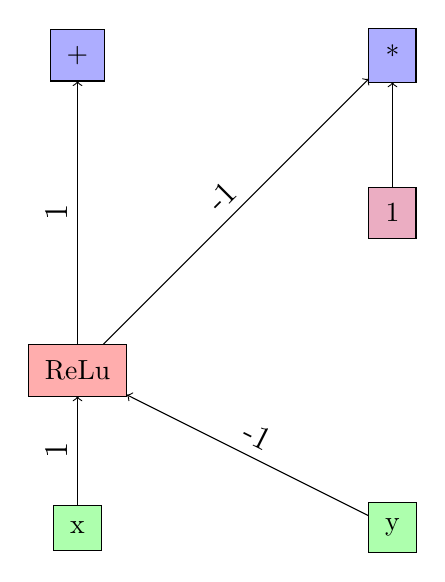
\begin{tikzpicture}
			
			
			\tikzstyle{input} = [shape=rectangle, draw, outer sep=0,inner  sep=6,minimum size=15, fill = green!32]
			\tikzstyle{hidden} = [shape=rectangle, draw, outer sep=0,inner  sep=6,minimum size=15, fill = red!32]
			\tikzstyle{bias} = [shape=rectangle, draw, outer sep=0,inner  sep=6,minimum size=15, fill = purple!32]
			\tikzstyle{output} = [shape=rectangle, draw, outer sep=0,inner  sep=6,minimum size=15, fill = blue!32]
			\tikzstyle{weight} = [thick,midway,sloped,above,->]
			
			\node[input] (i1) at (0,0) {x};
			\node[input] (i2) at (4,0) {y};
			
			\node[hidden] (h1) at (0,2) {ReLu};
			
			\node[bias] (b1) at (4,4) {1};
			
			\node[output] (o1) at (0,6) {+};
			\node[output] (o2) at (4,6) {*};			
			
			\draw[->](i1) -> (h1) node[weight] {\large 1};
			\draw[->](i2) -> (h1) node[weight] {\large -1};
			
			\draw[->](h1) -> (o1) node[weight] {\large 1};
			\draw[->](h1) -> (o2) node[weight] {\large -1};
			
			\draw[->](b1) -> (o2) node[weight] {};
			
			\end{tikzpicture}
			
			\caption{A 'router' network that abides by the standard structure of a feed-forward Neural Network}
			
		\end{figure}
		
		The above network demonstrates awareness of the function it computes because the neurons that correspond to either addition or multiplication will receive a zero or non-zero input depending on whether or not its function is to be used. Going forward, we will say that a neuron which receives an input of zero is 'inactive' and one which receives a non-zero input is 'active'. Of course, given different input values to the network, different neurons may become active or inactive. 
	
	\subsection{Manipulating symbols}
	
		Within the standard model of Neural Networks (neurons with activation functions that are interconnected by weights), manipulation of numerical values is commonplace. Manipulation of symbols, on the other hand. In the context of ANN's, a symbol is an internal state of some group of neurons. For example, when processing an input of an image, some neurons may compute a larger activation value if some feature exists in the input, so the region of inputs that corresponds to the existence of the feature 'symbolizes' that feature. The representations expressed by Symbols are categorical, such that some function (which will differ in different symbols) exists that maps the set of activities of the neurons in the group to a category. Symbols are a useful construct for identifying the underlying meaning behind each computation in a Neural Network.
		
		In figure 13 (section 2.9), a simple network either adds or multiplies two input values depending on which is greater. We can say that the group of the two output neurons (one being an adder and one a multiplier) is a symbol, which represents the function that was performed. The categorization function would simply check which activity is higher in each of the two neurons and will say that the symbol represents the function of whichever has the higher activity.
		
		\begin{figure}
	
	\centering
		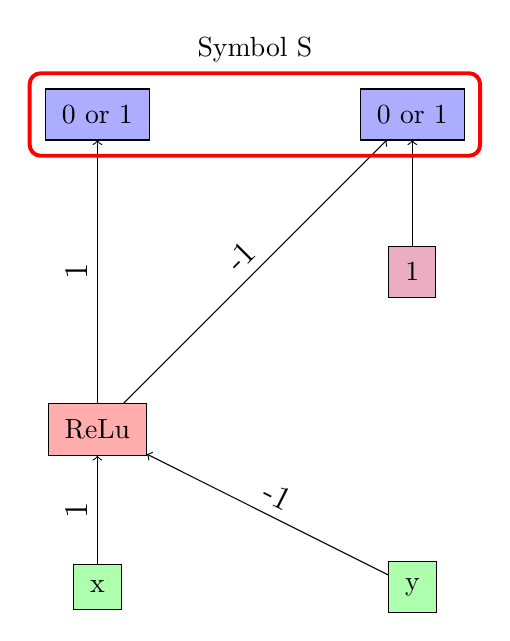
\begin{tikzpicture}
		
			
			\tikzstyle{input} = [shape=rectangle, draw, outer sep=0,inner  sep=6,minimum size=15, fill = green!32]
			\tikzstyle{hidden} = [shape=rectangle, draw, outer sep=0,inner  sep=6,minimum size=15, fill = red!32]
			\tikzstyle{bias} = [shape=rectangle, draw, outer sep=0,inner  sep=6,minimum size=15, fill = purple!32]
			\tikzstyle{output} = [shape=rectangle, draw, outer sep=0,inner  sep=6,minimum size=15, fill = blue!32]
			\tikzstyle{weight} = [thick,midway,sloped,above,->]
			
			\node[input] (i1) at (0,0) {x};
			\node[input] (i2) at (4,0) {y};
			
			\node[hidden] (h1) at (0,2) {ReLu};
			
			\node[bias] (b1) at (4,4) {1};
			
			\node[output] (o1) at (0,6) {0 or 1};
			\node[output] (o2) at (4,6) {0 or 1};			
			
			\draw[->](i1) -> (h1) node[weight] {\large 1};
			\draw[->](i2) -> (h1) node[weight] {\large -1};
			
			\draw[->](h1) -> (o1) node[weight] {\large 1};
			\draw[->](h1) -> (o2) node[weight] {\large -1};
			
			\draw[->](b1) -> (o2) node[weight] {};
			
			\node[draw,rounded corners,color=red,line width=0.5mm,inner sep=2mm,label=above:Symbol S,fit=(o1) (o2) (o1) (o2)] {};
		
		\end{tikzpicture}
		
		The corresponding definition of Symbol S is the following:
		
		\[ S =
		\begin{cases} 
			'Addition' & [1,0] \\
			'Multiplication' & [0,1]
		\end{cases}
		\]
		
		\caption{A 'router' network expressed using a Symbol}
		
	\end{figure}
	
	\section{Results}
	
	\section{Conclusions}
	
	\begin{thebibliography}{9}
		\bibitem{latexcompanion} 
		Sample reference 
	\end{thebibliography}

\end{document}

